\begin{figure}[htbp]
\centering
\begin{subfigure}[b]{0.95\textwidth}
\centering
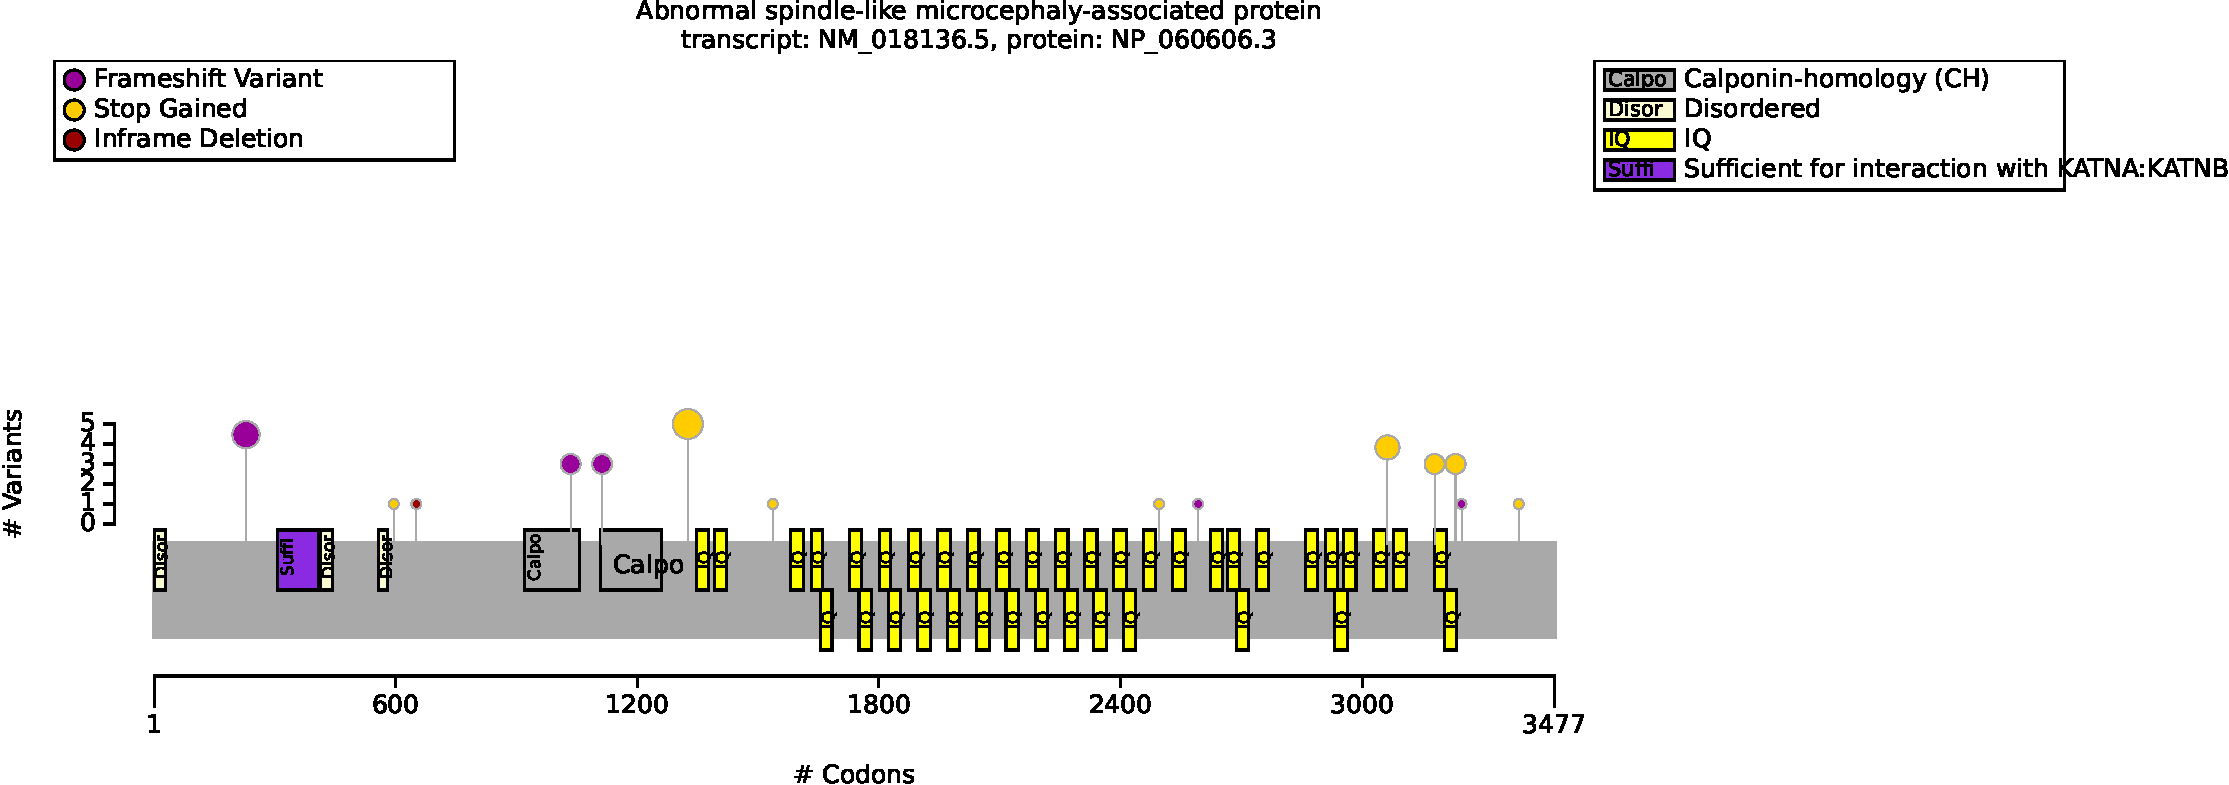
\includegraphics[width=\textwidth]{ img/ASPM_protein_diagram.pdf} 
\captionsetup{justification=raggedright,singlelinecheck=false}
\caption{Distribution of variants in ASPM}
\end{subfigure}

\vspace{2em}

\begin{subfigure}[b]{0.95\textwidth}
\centering
\resizebox{\textwidth}{!}{
\begin{tabular}{llllrr}
\toprule
Genotype (A) & Genotype (B) & total tests performed & significant results\\
\midrule
N Term/N Term OR N Term/other & other/other & 11 & 0\\
FEMALE & MALE & 11 & 0\\
\bottomrule
\end{tabular}
}
\captionsetup{justification=raggedright,singlelinecheck=false}
\caption{Fisher Exact Test performed to compare HPO annotation frequency with respect to N Term/N Term OR N Term/other and other/other, as well as male/female comparison. }
\end{subfigure}

\vspace{2em}

\caption{ The cohort comprised 22 individuals (14 females, 8 males). A total of 17 HPO terms were used to annotate the cohort. Disease diagnosis: Microcephaly 5, primary, autosomal recessive (OMIM:608716). No statistically significant results identified. A total of 28 unique variant alleles were found in \textit{ASPM} (transcript: \texttt{NM\_018136.5}, protein id: \texttt{NP\_060606.3}).}
\end{figure}
